\documentclass[../main.tex]{subfiles}

\begin{document}

\section{Redesign}

Having proven that the baseline design fails both in yield and in fatigue by significant margins, a redesigned torque arm with increased thickness is required.
Note that the peak Gerber value was greater than 5 for the baseline design.
A proposed redesign is as follows: increase the thickness of the body and bushing of the torque arm by a factor of 5 each, resulting in a body thickness of \(30\,\unit{\milli\meter}\) and a bushing thickness of \(40\,\unit{\milli\meter}\).
For this case we maintain the same boundary condition and unique steps for each load case, but adjust the magnitude of the traction so that the constant value of load for each case is maintained.
Based on the increased thickness of the bushing, the new tractions for preload and oscillating load are \(2.24\,\unit{\mega\pascal}\) and \(0.45\,\unit{\mega\pascal}\) respectively.
Again, the converged mesh from the baseline is used, with differing thickness represented in the plane stress section property options.
The CPS8R element type is also maintained for its speed and accuracy of modeling complex stresses throughout the torque arm. 

New Von Mises stress contours for the redesigned part are shown in figures \ref{redesigned_axial_mises}-\ref{redesigned_vertical_mises}.
The peak magnitude of stress for each step is significantly reduced compared to the baseline design. 
Note that the contour plots of stresses look identical to the baseline plots, although the maximum values are much smaller.
This result is valid for the way we are modeling the problem where the stress values are a direct function of the thickness of the part.
The critical stress regions are, once again, not located in the bushing, so our modeling assumptions from the baseline case hold equally valid.

\begin{figure}[H]
    \centering
    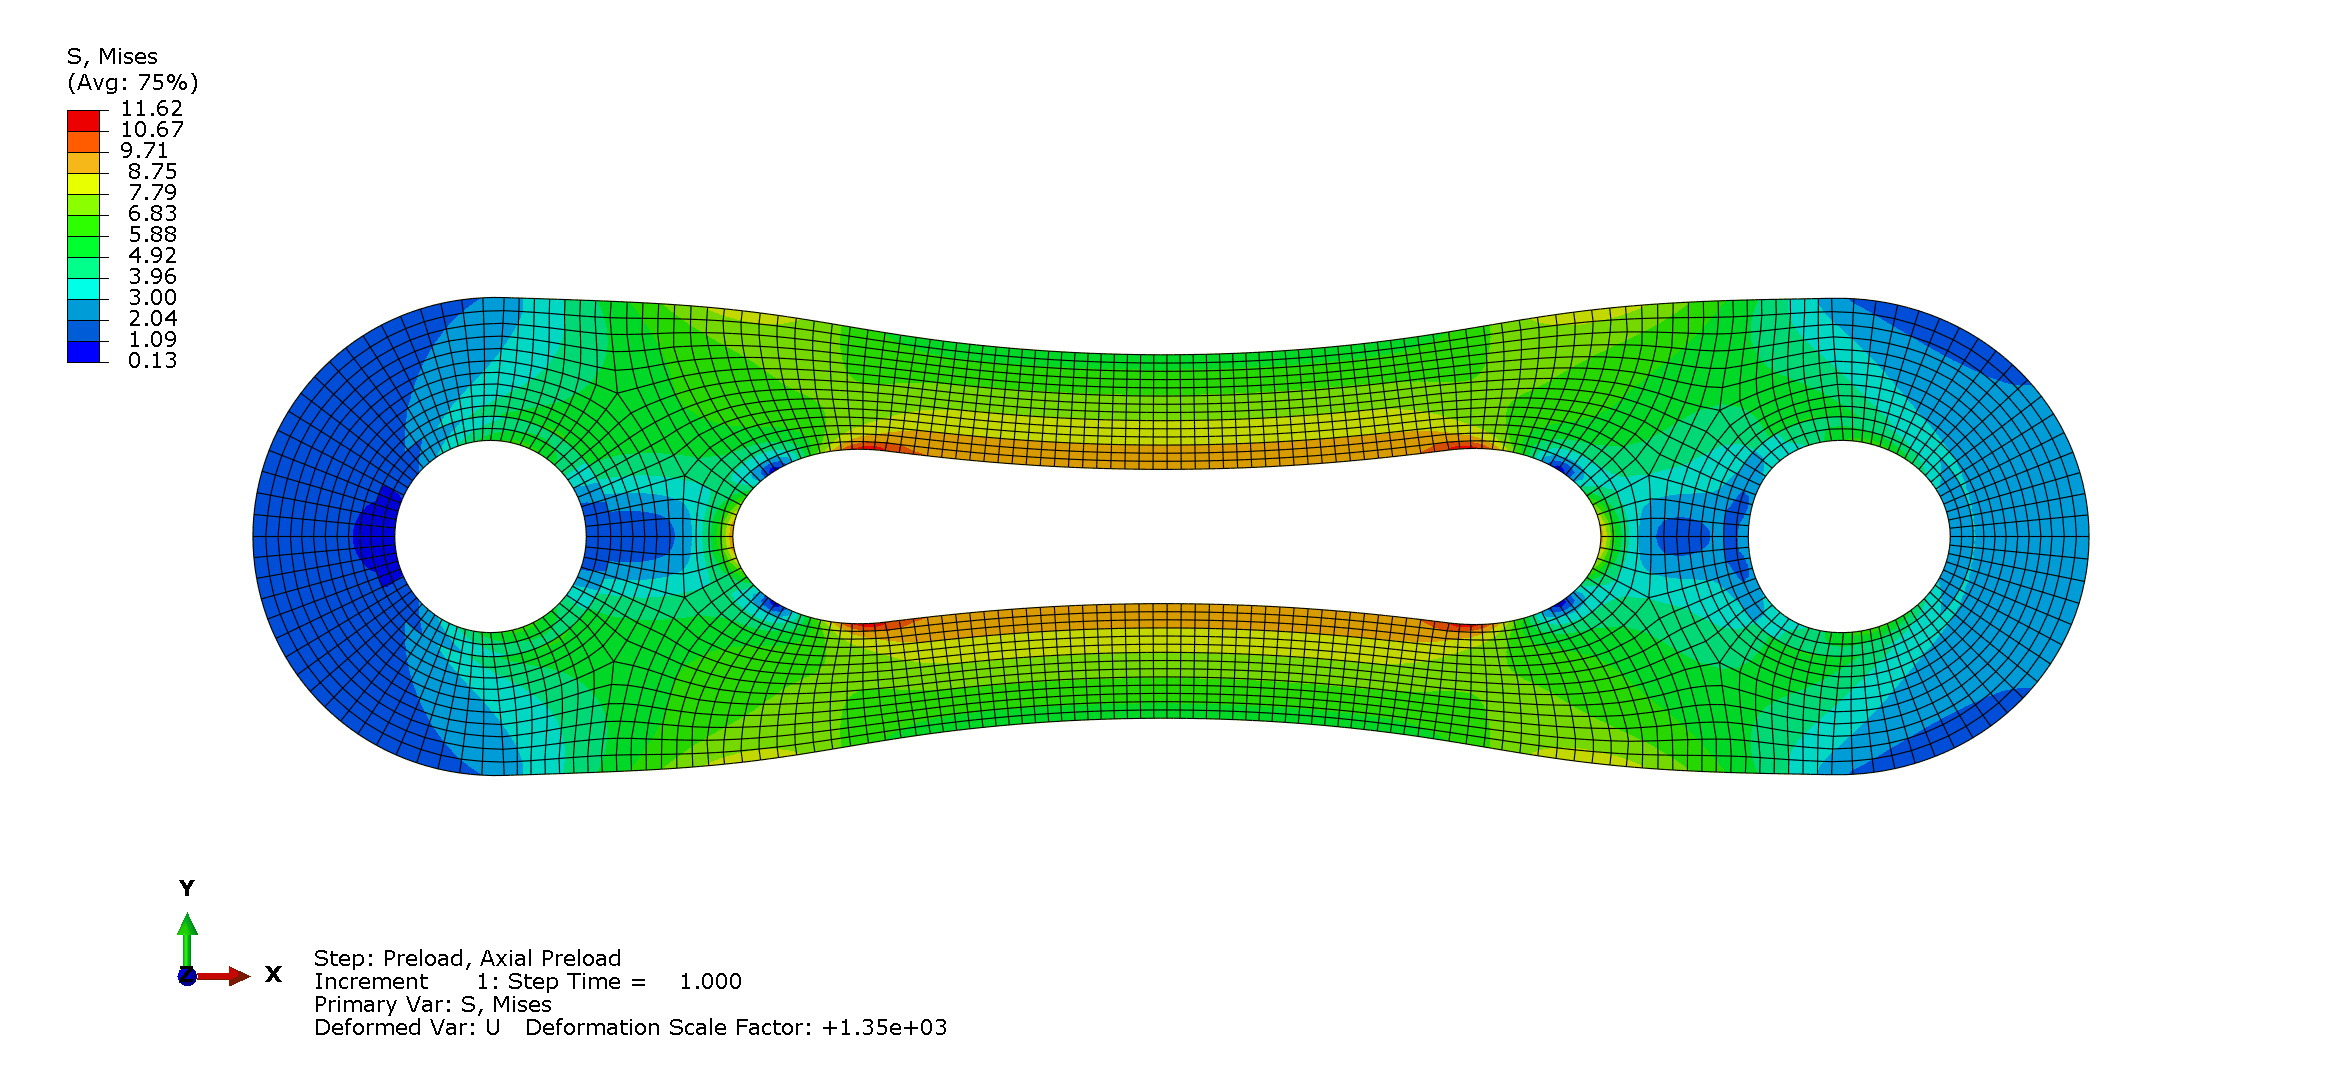
\includegraphics[scale=0.2]{../../images/40bush_30body_axial_mises.png}
    \caption{Contours of Von Mises stress for redesigned preload}
    \label{redesigned_axial_mises}
\end{figure}

\begin{figure}[H]
    \centering
    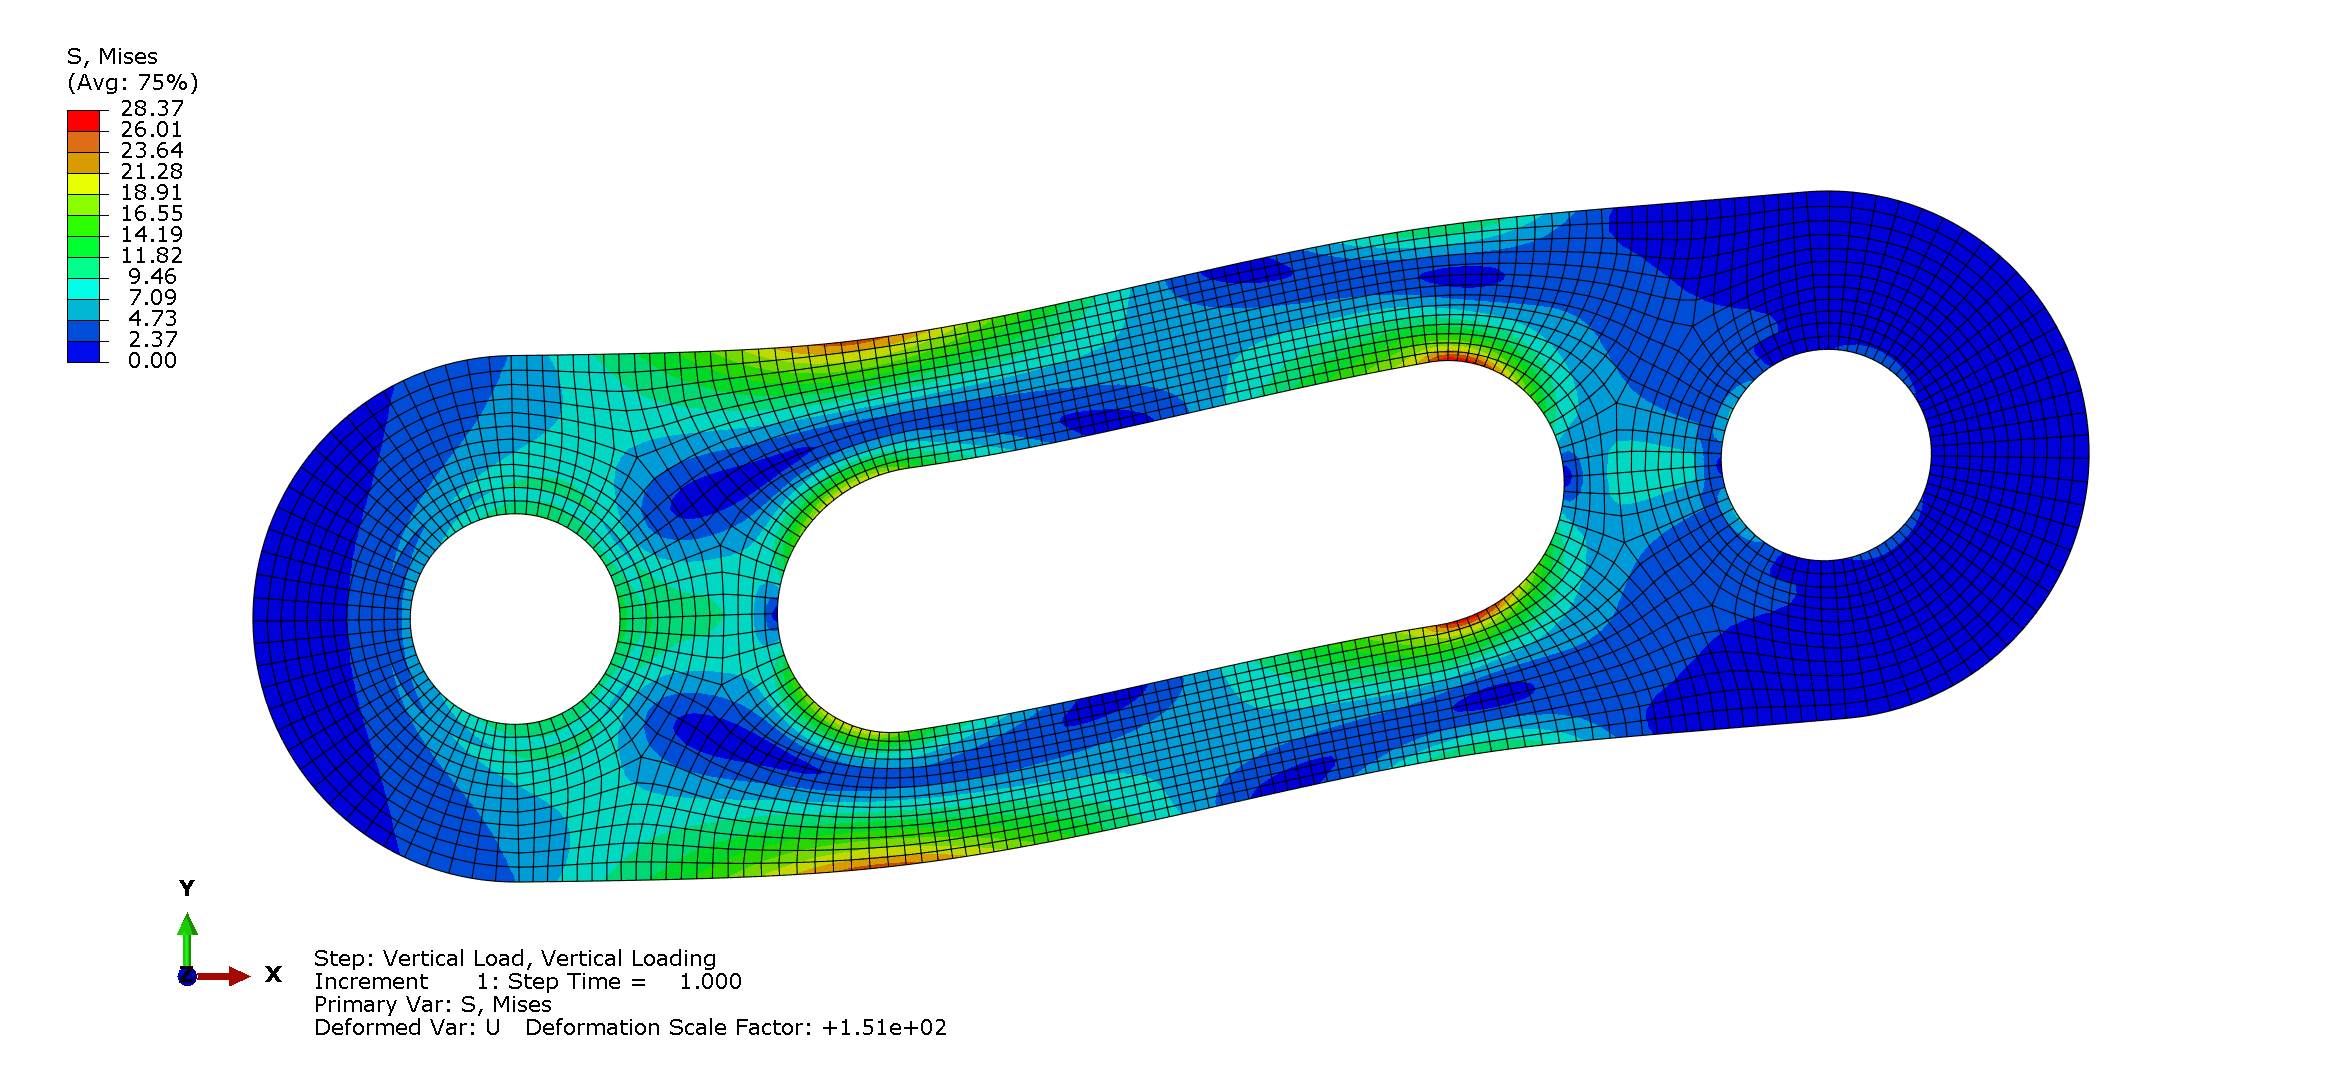
\includegraphics[scale=0.2]{../../images/40bush_30body_vertical_mises.png}
    \caption{Contours of Von Mises stress for redesigned oscillating load}
    \label{redesigned_vertical_mises}
\end{figure}

Next, we examine the torque arm's yield performance. 
Combining the Von Mises stress contours again and comparing to the yield strength, we see that the redesigned part does not experience a failure from yield, with all stresses below \(75\,\unit{\mega\pascal}\).
The maximum stresses occur in the same locations as the baseline design with a reduced amplitue, shown in figure \ref{redesigned_combined_mises}.


\begin{figure}[H]
    \centering
    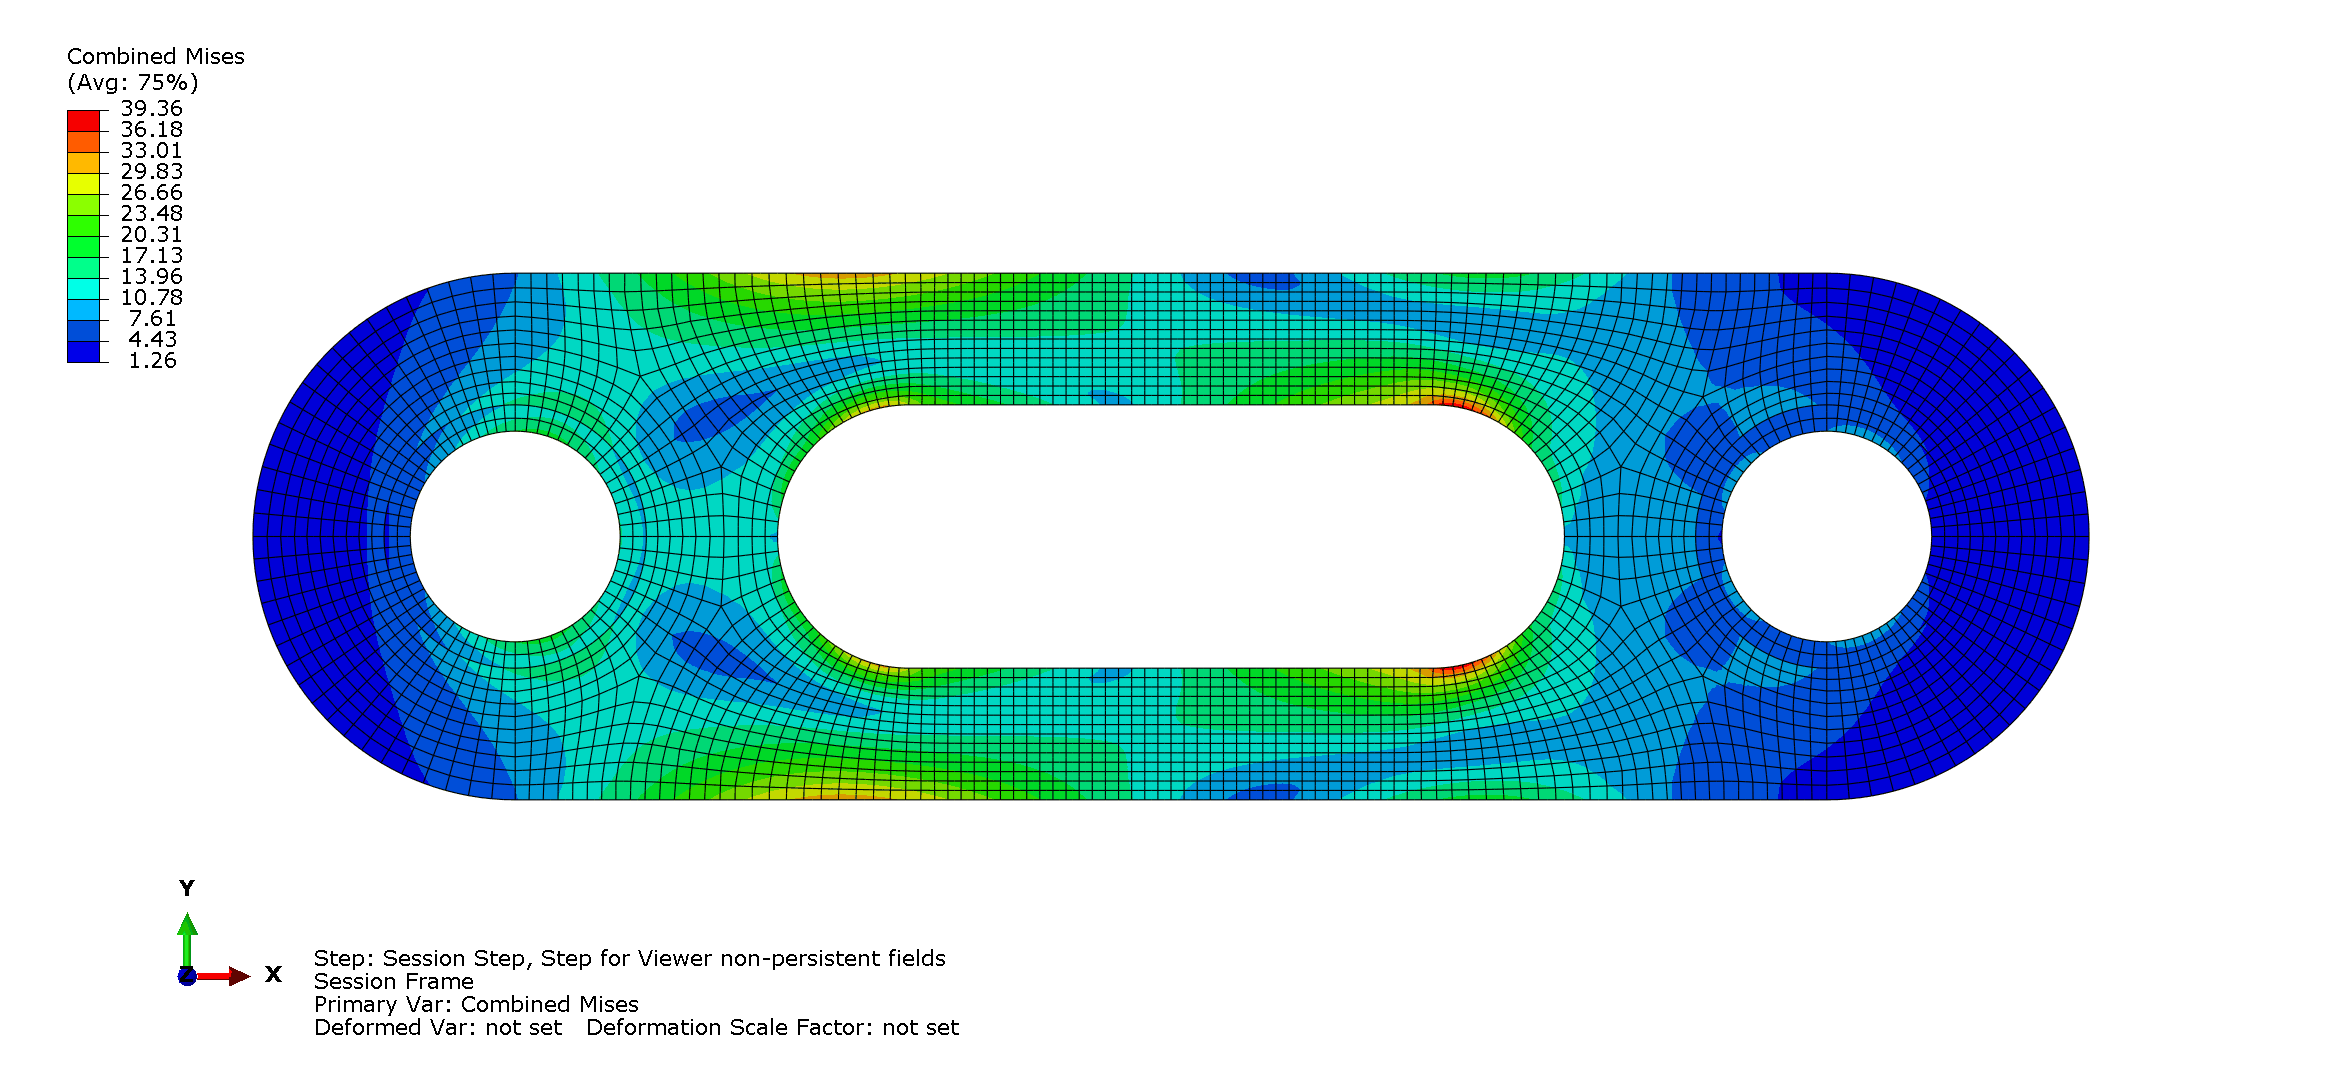
\includegraphics[scale=0.2]{../../images/40bush_30body_combined_mises.png}
    \caption{Contour plot of combined Von Mises stresses on redesigned model}
    \label{redesigned_combined_mises}
\end{figure}

The baseline design was much more likely to fail from fatigue than from yield, so evaluation of the Gerber values for the redesigned part is especially important.
Figure \ref{redesigned_gerber} shows a peak Gerber value of 0.97, 3\% from the limit of 1.
The redesigned part is overly strong in yield but fairly close to the fatigue design limit.
A fatigue failure would appear at the bottom right of the center gap, where the peak value of 0.97 is observed.

\begin{figure}[H]
    \centering
    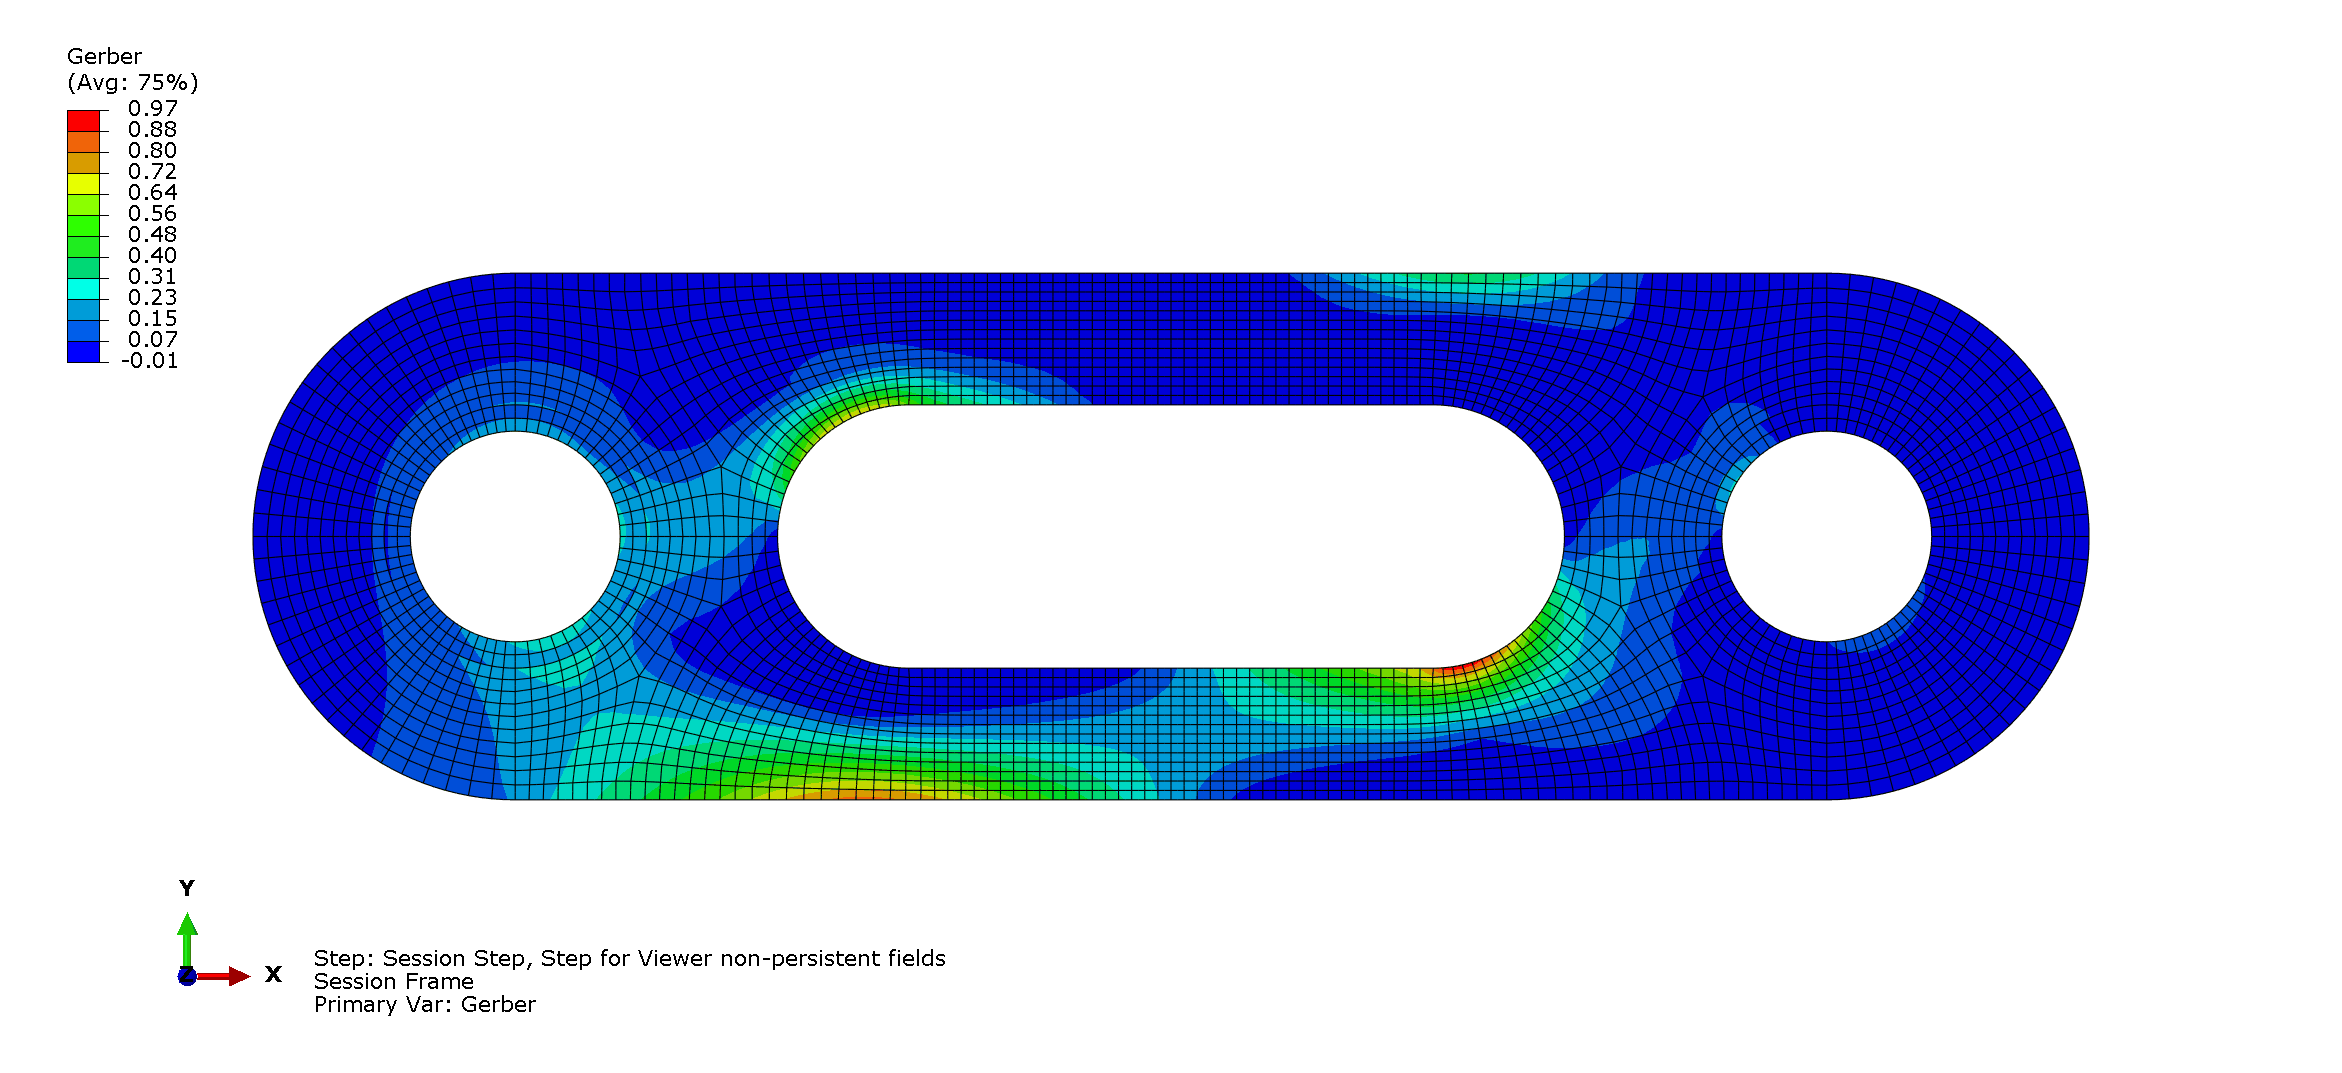
\includegraphics[scale=0.2]{../../images/40bush_30body_gerber.png}
    \caption{Contour plot of Gerber equation values on redesigned model}
    \label{redesigned_gerber}
\end{figure}

Based on the Von Mises and Gerber criteria examined we have redesigned the part to no longer experience the same failure modes of the baseline.
The redesigned part has a safety factor of \(n=1.02984\), indicating that is very close to the failure threshold (for details, see appendix \ref{safety}).
The thickness increases a dramatic amount and a better method of redesign could potentially be to use a different material with a larger modulus of elasticity.
However, if the part is primarily weight-constrained rather than volume constrained, an increase in thickness may be a valid avenue rather than using a denser material.



\end{document}



